\chapter{Background and inspiration}

\epigraph{It has to start somewhere \\ it has to start sometime \\ what better place than here? \\ what better time than now?}{Guerrilla Radio \\ Rage Against the Machine, 1999}

\section{Microcontrollers as alternative to computers}

When I joined MIT Media Lab in 2019, I made the decision to focus my efforts on hardware research, so I could make computational art devices, instead of software that needs to run on a laptop computer or a browser. This was fueled by the introduction of restrictive news by Apple, such as advising against the use of apps created by unregistered developers and discontinuing support for 32-bit apps, and by the ever-changing nature of the web, which makes my online artwork break often and need maintenance, and the need for additional corporate infrastructure to keep it online. In contrast I saw hardware as a space where I could deploy my ideas and keep them running without outside intervention.

I started my research by catching up with the newer developments by Teensy. The newer microcontrollers are faster and more powerful, and I used them to design and implement many small projects. I want to mention this personal project, a standalone audiobook I made with rotary encoders and a small screen for navigation, because it led me to include software for support of this same screen in the TinyTrainable library.

\begin{figure}[ht]
  \centering
  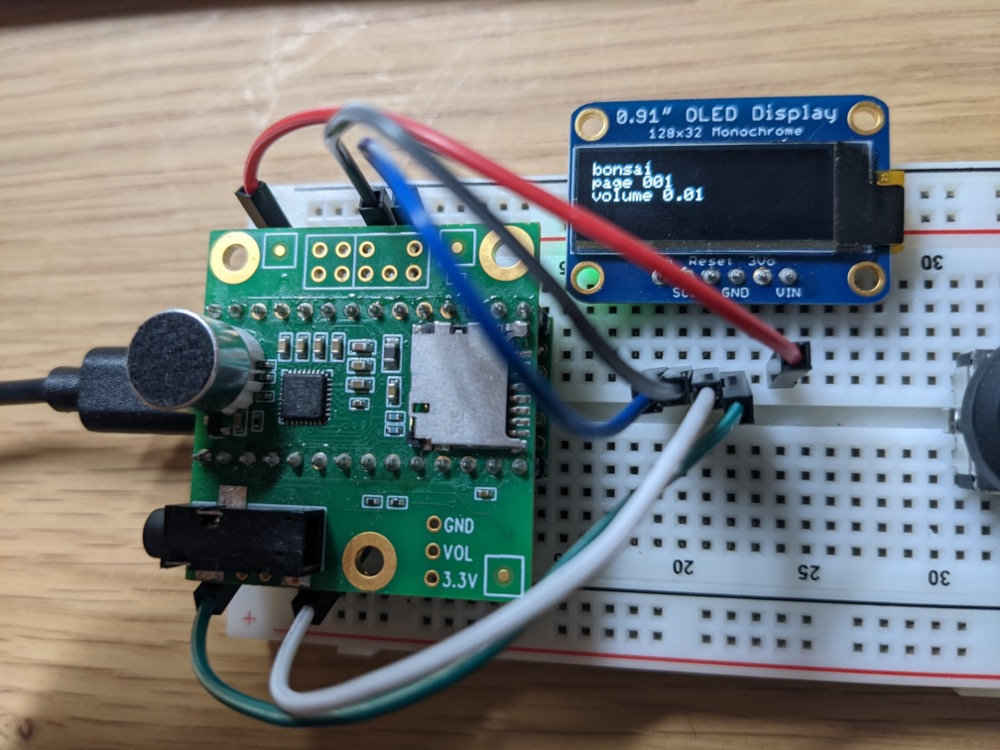
\includegraphics[width=0.75\linewidth,height=0.40\textheight,keepaspectratio]{images/bonsai.jpg}
  \caption{Audiobook made with Teensy}
  \caption*{Picture taken by myself}
  \label{fig:bonsai-audiobook}
\end{figure}

In parallel, I researched the evolution of the teaching of physical computing at \acrshort{NYU} \acrshort{ITP}, and I discovered that they stopped teaching with the now classic Arduino Uno, and have replaced it with the newer series of Arduino Nano microcontrollers, which have a smaller format and and operating voltage of 3.3V instead of 5V.

While browsing this series, I discovered the Arduino Nano 33 \acrshort{BLE} Sense that I based my thesis now. It comes with 9 emedded sensors, to measure and detect acceleration, movement, distance, color, and a microphone. This is an amazing help for beginners, since a huge challenge when you are starting to build your own projects and learning electronics, is reading datasheets to understand what sensors you can use with your microcontroller, how to wire them and callibrate them, and then what library supports it. This makes it easier and cheaper to prototype, and this made my work on my thesis easier, since I didn't have to include instructions for wiring sensors or callibrating them, and I could focus on \acrshort{ML} and the different outputs for arts.

\section{Coursework at MIT}

As part of the research that directly inspired this thesis, here is the coursework I took, and my notes about how they inform my theoretical and practical background for Tiny trainable instruments.

\begin{enumerate}
  \item Fall 2019, CMS.901 Current Debates in Media, by professor Sasha Costanza-Chock
  \item Fall 2019, MAS.S65 Recreating The Past, by professor Zach Lieberman
  \item Spring 2020, MAS.826 Sound: Past and Future, by Tod Machover
  \item Spring 2020, MAS.712 Learning Creative Learning, by professor Mitchel Resnick
\end{enumerate}

In the class Current Debates in Media, topics covered included fake news, surveillance, algorithmic bias, data colonialism, climate justice, algorithms of oppression, among others. For my final paper I wrote on the role of the media during the 2019 Chilean protests. This class directly inspired me to look for privacy-first \acrshort{ML}, and thinking about \acrshort{AI} in a critical way and not as clean safe automation, but as invisibilized labor, exploitation, and algorithmic bias and discrimination in the worst scenarios.

In the class Recreating the Past, I learned about media arts history, and I dived deep in the language C++ which I used for writing the TinyTrainable library, while working with the library openFrameworks, which is one of the most popular open source frameworks and communities for media arts.

In the class Sound: Past and Future, I learned more about the history of different computational advancements for sound, with a strong focus on projects at MIT Media Lab's own research groups including Opera of the Future, Hyperinstruments, and Music, Mind, and Machine. This class introduced me to many projects and it helped me decide on making instruments for my thesis, using the latest technologies I could find, in this case, microcontrollers and \acrshort{ML}.

In the class Learning Creative Learning, I was introduced to the Lifelong Kindergarten's frameworks and ideas, including the 4 P's (peers, projects, passion, and play), and the design of Scratch as a home with low floor, wide walls, and high ceiling, which I highly recommend to check on Mitchel Resnick's book Lifelong Kindergarten. This class gave me the push to write a library with a community in mind, starting with the development of it, which happened because I had the pleasure of working with MIT undergrads Peter Tone and Maxwell Wang, who helped me with different aspects of research and development.

\section{Research projects at MIT}

Some other projects I created during this master's include:

\begin{enumerate}
  \item SiguesAhi: an instrument to detect when oppressive institutions have ceased to exist. It is achieved with microcontrollers with Internet connectivity.
  \item Open Drawing Machine, with Gaurav Patekar: an open source low cost programmable drawing machine
  \item Introduction to networks for artists: a series of tutorials for beginners, to learn how to set up their own networks and collaborate in peer-to-peer ways for making art.
\end{enumerate}

SiguesAhi is a sibling project to Tiny trainable instruments. It is based on a microcontroller from the same series and format but different architecture and capabilities, the Arduino Nano 33 IoT.

\begin{figure}[ht]
  \centering
  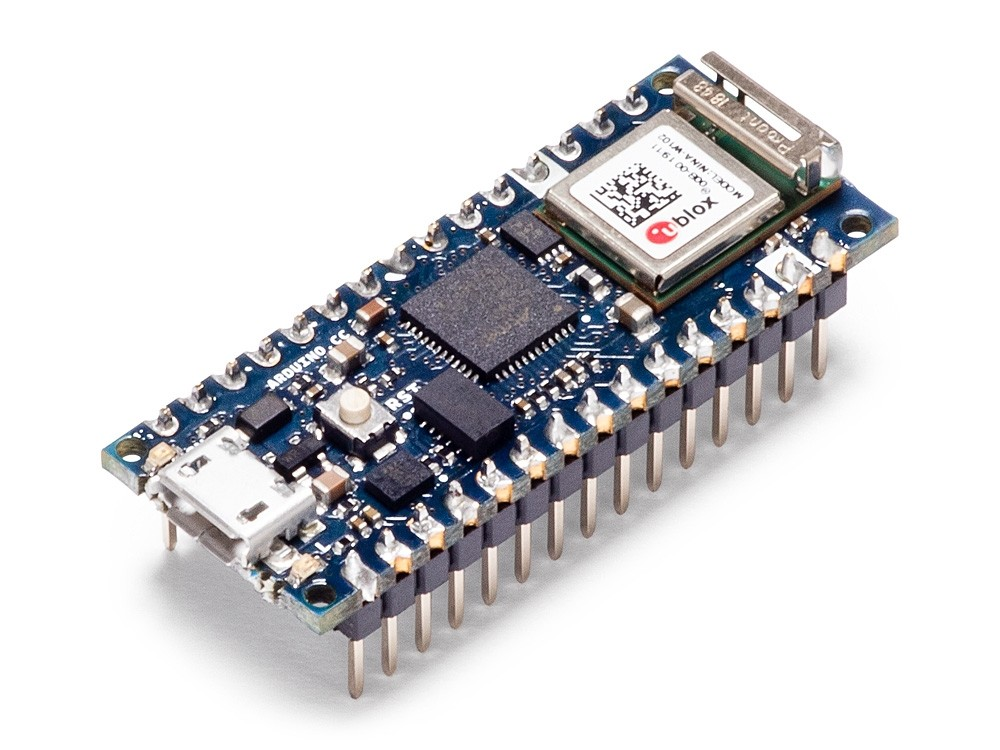
\includegraphics[width=0.75\linewidth,height=0.25\textheight,keepaspectratio]{images/arduino-nano-33-iot-with-headers.jpg}
  \caption{Arduino Nano 33 IoT with headers}
  \caption*{Retrieved from \cite{website-arduino-nano-33-iot-with-headers}}
  \label{}
\end{figure}

For this project, I am writing a library for making digital instruments that can detect if institutions still exist. This is accomplished by connecting the microcontroller to the internet, and making it ping the Wikipedia website with a certain periodicity, in order to download and check the first sentence of the first paragraph of the entry. As an example of the library, I am using the National Rifle Association, which sadly still exists.

\begin{figure}[ht]
  \centering
  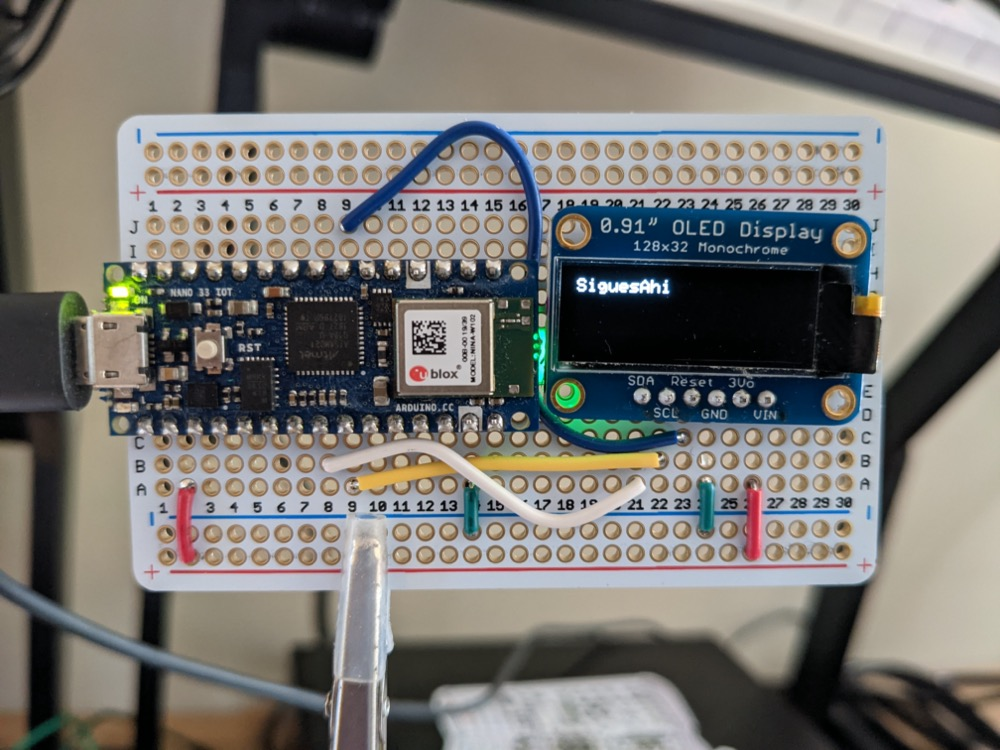
\includegraphics[width=0.75\linewidth,height=0.25\textheight,keepaspectratio]{images/siguesahi.jpg}
  \caption{SiguesAhi project}
  \caption*{Picture by myself}
  \label{fig:siguesahi}
\end{figure}

The \cite[Open Drawing Machine]{website-open-drawing-machine} is a collaborative project with Gaurav Patekar for the research group Future Sketches at MIT Media Lab. It is a low cost open source machine, consisting of an Arduino microcontroller and hardware for drawing computationally. We have done the research together, Gaurav designed and 3D printed the hardware, and I have packaged the results as a still unfinished openFrameworks addon.

\begin{figure}[ht]
  \centering
  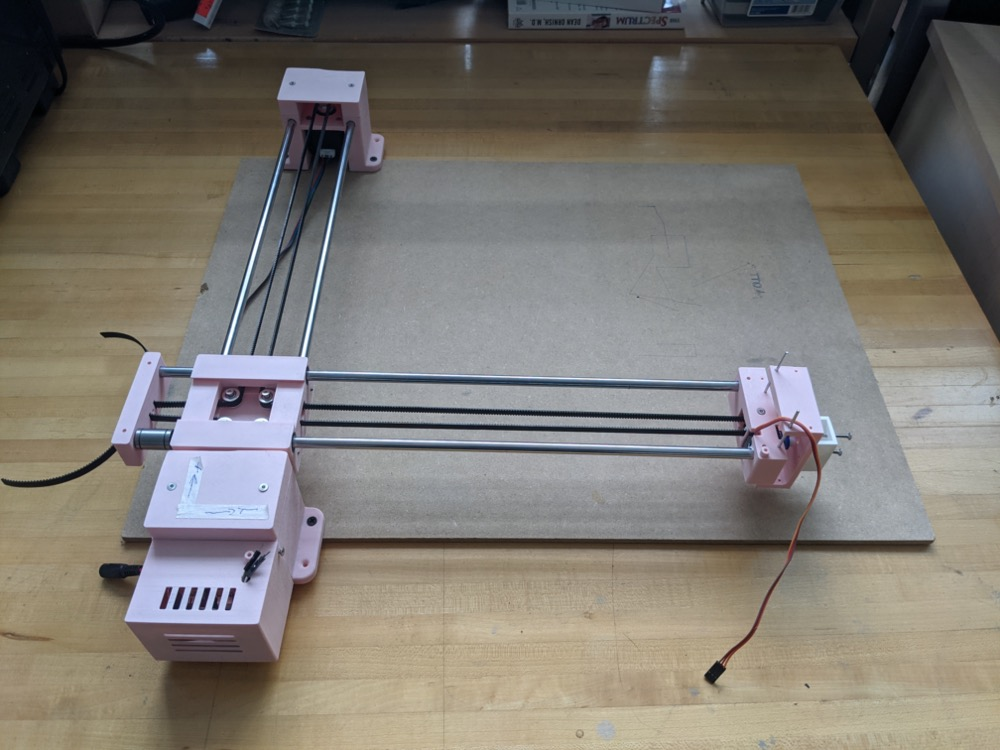
\includegraphics[width=0.75\linewidth,height=0.25\textheight,keepaspectratio]{images/open-drawing-machine.jpg}
  \caption{Open Drawing Machine project}
  \caption*{Picture by myself}
  \label{fig:open-drawing-machine}
\end{figure}

Currently the Open Drawing Machine can receive drawing commands from a computer through a serial port, and the next step of this project is being able to receive commands from other computers through networks and the internet. This comes from the last project I will mention that I worked on while at MIT Media Lab, which is Introduction to computer networks for artists \cite{website-intro-to-computer-networks-for-artists}, a collection of tutorials for remote peer-to-peer collaboration between artists. This project is inspired by the amazing research on remote collaboration, sensors, peer-to-peer protocols, by friend Lisa Jamhoury, including the app Kinectron.

\begin{figure}[ht]
  \centering
  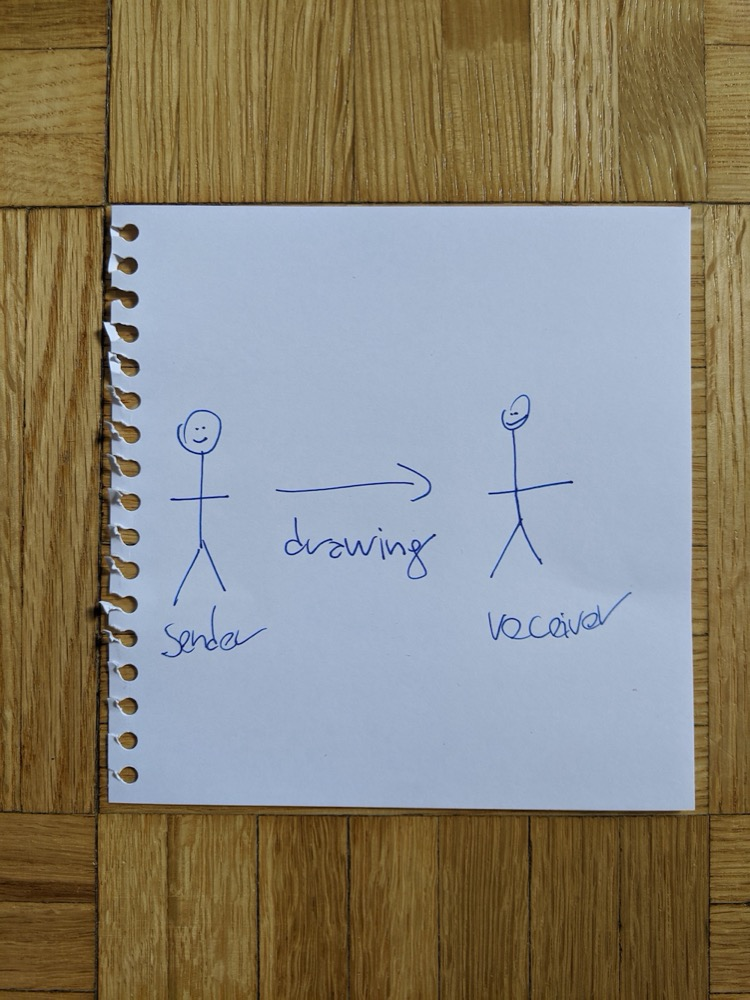
\includegraphics[width=0.75\linewidth,height=0.35\textheight,keepaspectratio]{images/intro-to-computer-networks-for-artists.jpg}
  \caption{Introduction to computer networks for artists project}
  \caption*{Picture by myself}
  \label{fig:intro-to-computer-networks-for-artists}
\end{figure}

\section{Computational media arts instruments}

There is a rich ecosystem of personal computers, operating systems and software for making art, and it is common nowadays for artists to rely on their computer for making all of their art, on the go, wherever they are. In the 1990s, musicians stopped having to rely on analog hardware, and started replacing their tools for recording and mixing with software on their computers.

Apart from the proliferation of laptop computers and software for arts, I will share my research in devices that I like to call computational media arts instruments. They are computational because they are digital and crunch numbers, and they are instruments that allow us to process different media in creative ways.

I will focus on the instruments that can be programmed, and that promote open source hardware or software. Many of these instruments often sit at my desk for inspiration, or I spend hours playing with them for my art and learning from them and the communities around them.

The tables \ref{table:media-arts-instruments-technical} and \ref{table:media-arts-instruments-influence} are respectively summaries of techniques and influences of the instruments that I reference in this section.

\begin{table}[ht]
    \centering
    \begin{tabular}{ | l |  l | l | l | l |}
        \hline
        Company             & Instrument    & Year  & Basis & Software            \\
        \hline
        Bastl Instruments   & Illuminati    & 2019  & MCU       & None                \\
        Bastl Instruments   & Kastle Drum   & 2020  & MCU       & Arduino, C++        \\
        Bastl Instruments   & Kastle v1.5   & 2017  & MCU       & Arduino, C++        \\
        Bastl Instruments   & OMSynth       & 2016  & IC        & None                \\
        Bastl Instruments   & microGranny 2 & 2016  & MCU       & Arduino, C++        \\
        Bastl Instruments   & Servo         & 2016  & MCU       & Arduino, C          \\
        Critter \& Guitari  & Organelle     & 2016  & Linux     & Pure Data           \\
        Critter \& Guitari  & EYESY         & 2020  & Linux     & Python, Pygame      \\
        monome              & aleph         & 2013  & Linux     & C                   \\
        monome              & norns         & 2018  & Linux     & Lua, SuperCollider  \\
        Shbobo              & Shnth         & 2013  & MCU       & Shlisp              \\
        Shbobo              & Shtar         & 2017  & MCU       & Shlisp              \\
        \hline
    \end{tabular}
    \caption{Technical details of media arts instruments}
    \label{table:media-arts-instruments-technical}
\end{table}{}

\begin{table}[ht]
    \centering
    \begin{tabular}{ | l |  l | l |}
        \hline
        Company             & Instrument    & Influence                             \\
        \hline
        Bastl Instruments   & Illuminati    & Output with LEDs                      \\
        Bastl Instruments   & Kastle series & Use of breadboard and jumper wires    \\
        Bastl Instruments   & OMSynth       & Distribution as tutorials + parts kit \\
        Bastl Instruments   & microGranny 2 & Arduino as basis for instrument       \\
        Bastl Instruments   & Servo         & Output with servo motor               \\
        Critter \& Guitari  & Organelle     & Computer for sound                    \\
        Critter \& Guitari  & EYESY         & Output with screen                    \\
        monome              & aleph, norns  & Computer for sound                    \\
        Shbobo              & Shnth, Shtar  & Input with multiple gestures          \\
        \hline
    \end{tabular}
    \caption{Influence of media arts instruments}
    \label{table:media-arts-instruments-influence}
\end{table}{}

\subsection{Bastl Instruments}

Bastl Instruments is a Czech company of multimedia instruments, which has had a huge impact and influence on my research and practice. When I first started researching the Eurorack format some years ago, I visited the shop Control in Brooklyn, NY, and some modules by Bastl stood out to me, because of their wooden panels and interaction with classic physical computing educational materials, such as motors and solenoids, which was an inspiration for me to include servo motors as an output in Tiny trainable instruments.

\begin{figure}[ht]
  \centering
  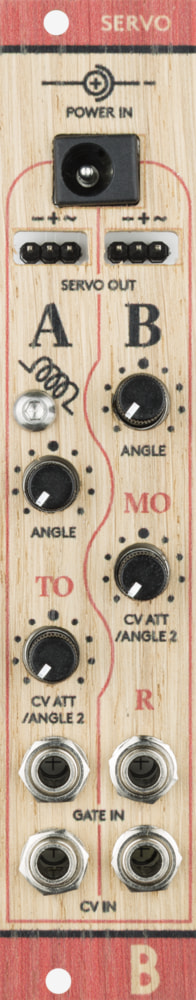
\includegraphics[width=0.75\linewidth,height=0.25\textheight,keepaspectratio]{images/bastl-servo.jpg}
  \caption{Bastl Instruments Servo module}
  \caption*{Retrieved from \cite{website-bastl-instruments-current}}
  \label{fig:bastl-servo}
\end{figure}

Another inspiration comes from their microgranny 2 granular sampler which is made with an Atmega microcontroller and its firmware is open source and available as a repository on their GitHub account, along with many other of their instruments.

\begin{figure}[ht]
  \centering
  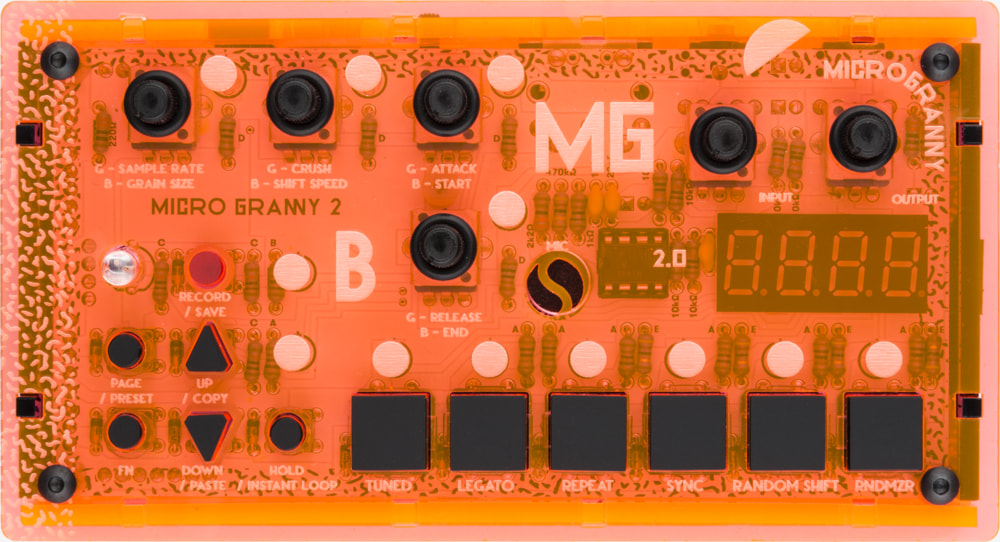
\includegraphics[width=0.75\linewidth,height=0.25\textheight,keepaspectratio]{images/bastl-microgranny-2.jpg}
  \caption{Bastl Instruments microGranny 2}
  \caption*{Retrieved from \cite{website-bastl-instruments-current}}
  \label{fig:bastl-microgranny-2}
\end{figure}

Their Kastle synthesizers are also based on microcontrollers, and feature a patchbay for making connections with jumper wires, the same used for prototyping in electronic breadboards, which influenced me to make the Tiny trainable instruments built with breadboards and jumper wires, instead of custom printed circuit boards. Also, the Kastle synths are forgiving instruments, their inputs and outputs are robust enough to allow for mistakes in connections, in an electrical and mechanical way, which I think is perfect for safe experimentation. It would be a bummer if the instrument was easy to break, or if it demanded a huge effort in understanding electronics for using it.

\begin{figure}[ht]
  \centering
  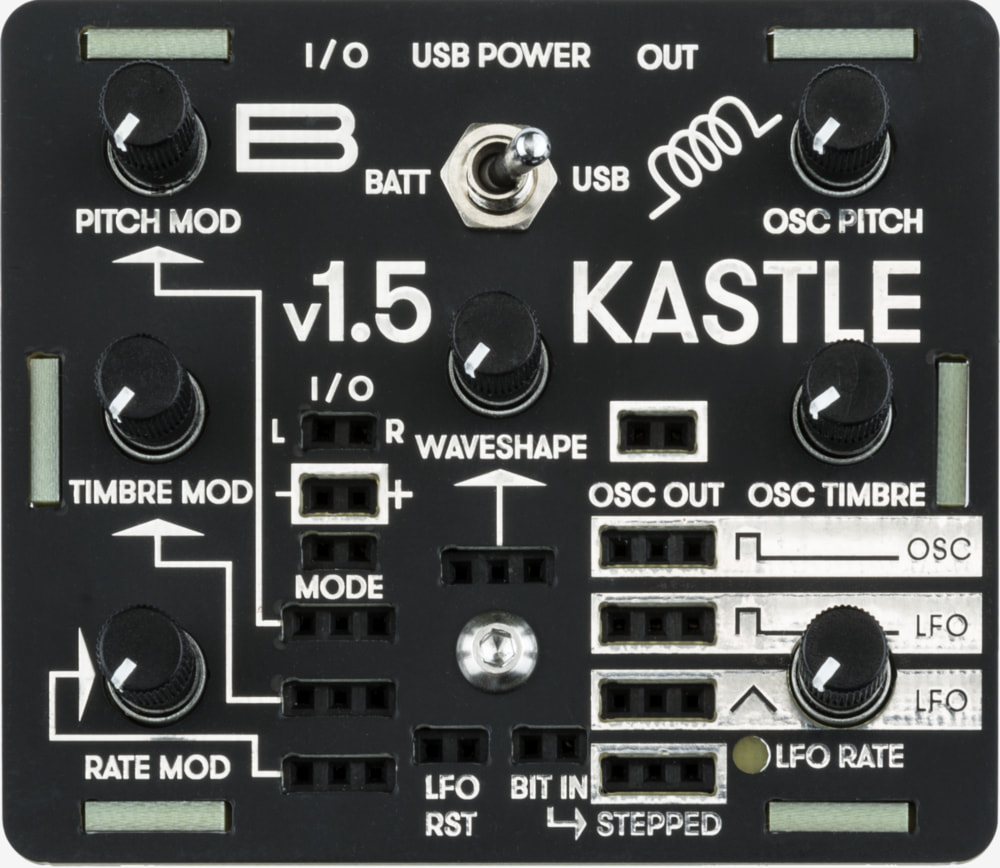
\includegraphics[width=0.75\linewidth,height=0.25\textheight,keepaspectratio]{images/bastl-kastle-v15.jpg}
  \caption{Bastl Instruments Kastle v1.5}
  \caption*{Retrieved from \cite{website-bastl-instruments-current}}
  \label{fig:bastl-kastle-v15}
\end{figure}

As of writing, two different units are in production, both retailing for around 100.00 USD: the Kastle v1.5 melodic / drone synthesizer, and the Kastle Drum, for rhythm. The only difference between these synthesizers is the firmware and the labels on the faceplate. The community is encouraged to write new firmware to modify their behavior. 

\begin{figure}[ht]
  \centering
  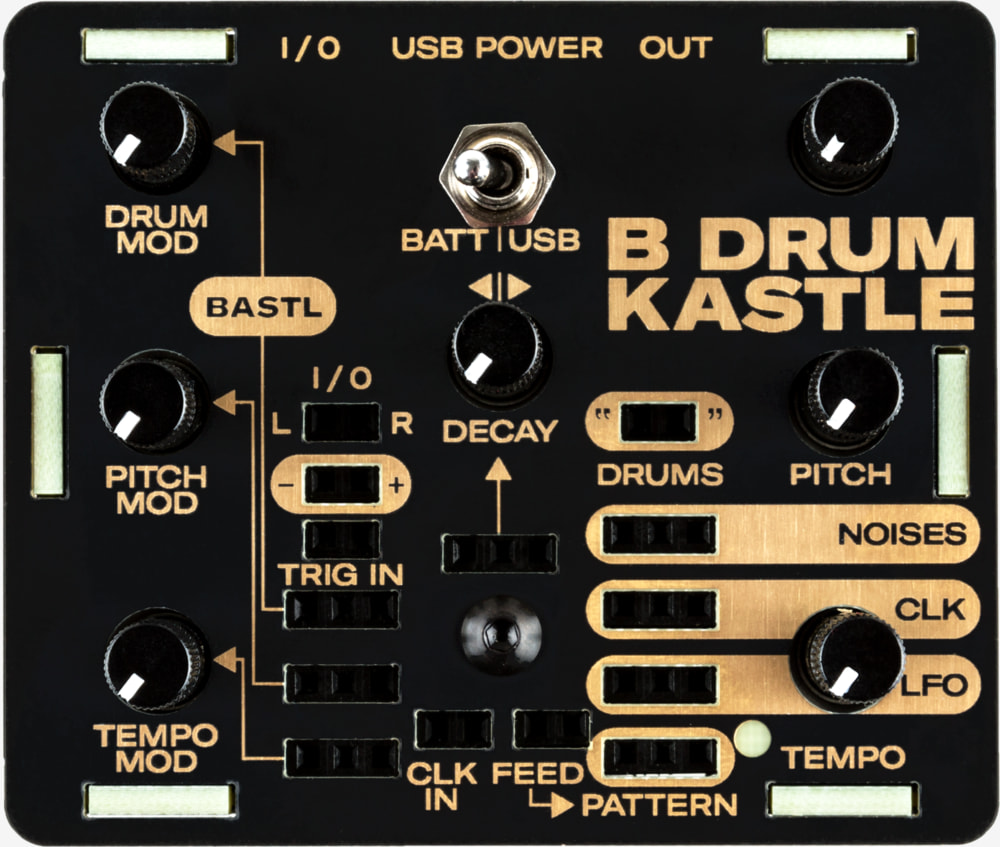
\includegraphics[width=0.75\linewidth,height=0.25\textheight,keepaspectratio]{images/bastl-kastle-drum.jpg}
  \caption{Bastl Instruments Kastle Drum}
  \caption*{Retrieved from \cite{website-bastl-instruments-current}}
  \label{fig:bastl-kastle-drum}
\end{figure}

Another instrument I want to highlight is the Illuminati, currently discontinued, a device that uses different inputs (audio, control voltage, \acrshort{MIDI} messages) to control the light intensity of connected USB lamps, which influenced the conception of Tiny trainable instruments as multimedia arts instruments, not only focusing on audio and music, but also printed text, light, and screen output.

\begin{figure}[ht]
  \centering
  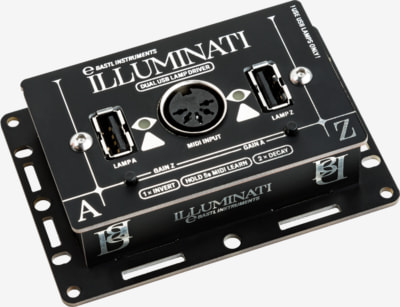
\includegraphics[width=0.75\linewidth,height=0.25\textheight,keepaspectratio]{images/bastl-illuminati.jpg}
  \caption{Bastl Instruments Illuminati}
  \caption*{Retrieved from \cite{website-bastl-instruments-current}}
  \label{fig:bastl-illuminati}
\end{figure}

The final instrument from this company that I want to highlight is the OMSynth, one of many collaborations with Casper Electronics. This device is an educational and maker circuit development tool for creating synthesizers. It includes basic fundamental blocks, such as battery power, audio input and output, potentiometers for attenuating and boosting signals, and a suite of parts kits for building devices including sequencers, oscillators, and samplers, on the included breadboard. Its release as a kit was also a direct influence in the release of Tiny trainable instruments as a kit with instructions.

\begin{figure}[ht]
  \centering
  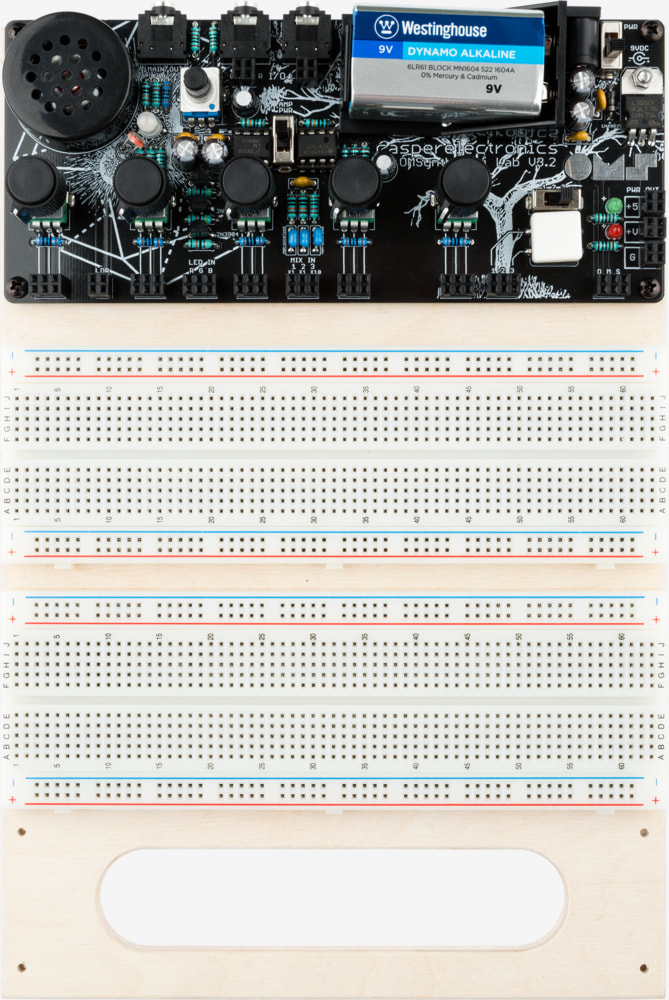
\includegraphics[width=0.75\linewidth,height=0.25\textheight,keepaspectratio]{images/bastl-omsynth.jpg}
  \caption{Bastl Instruments OMSynth}
  \caption*{Retrieved from \cite{website-bastl-instruments-current}}
  \label{fig:bastl-omsynth}
\end{figure}

Many BASTL standalone instruments are 200.00 USD or less, which is a huge contrast to the 1960s, when a Moog analog system II cost 6,200.00 USD, which was enough to buy a small house \cite{analog-days}. Also, many of their instruments are sold as kits for building and soldering them yourself, for the cheaper cost and the added educational aspect of having hands-on experience.

\subsection{Critter \& Guitari}

Critter \& Guitari is an American company based in Brooklyn NY, which has released in the past computational microcontroller-based audiovisual instruments, from which my favorite is the Kaleidoloop, currently discontinued. It is a sampler with an internal mic and speaker, that allows you to record audio and then control its output with 2 knobs for volume and playback rate. It is designed to be portable for doing field recordings, and it was an influence on the design of the Tiny trainable instruments library, which allows the construction of standalone instruments, that with a USB power bank or a battery, you can take for a walk or place anywhere you want.

\begin{figure}[ht]
  \centering
  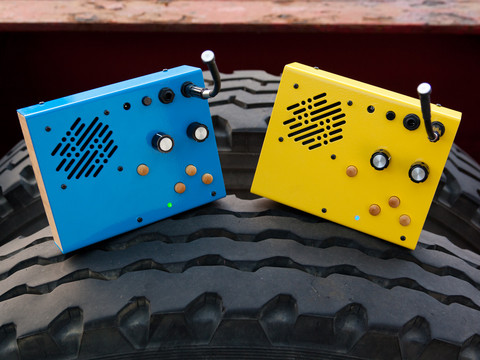
\includegraphics[width=0.75\linewidth,height=0.25\textheight,keepaspectratio]{images/critter-and-guitari-kaleidoloop.jpg}
  \caption{Critter \& Guitari Kaleidoloop}
  \caption*{Retrieved from \cite{website-critter-and-guitari-kaleidoloop}}
  \label{fig:critter-and-guitari-kaleidoloop}
\end{figure}

In 2015, Critter \& Guitari released the Organelle, a sound computer with the Linux operating system installed, and the software Pure Data as the programmable interface between the hardware and the sound engine. Every sound you can do on an Organelle you could do on your laptop using Pure Data too, and you could build your own interface to interact with the sound.

\begin{figure}[ht]
  \centering
  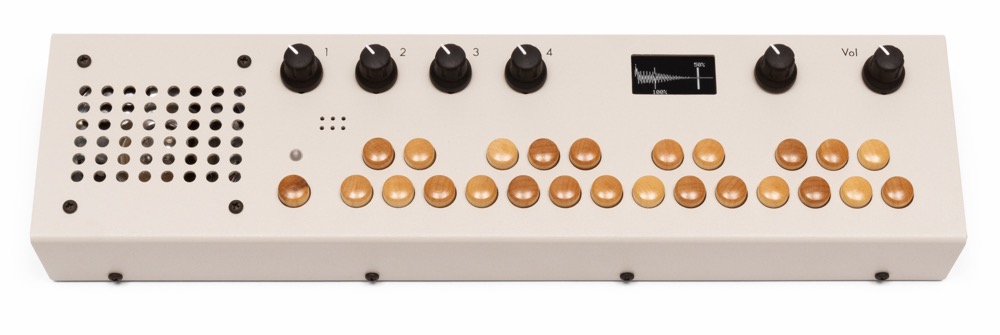
\includegraphics[width=0.75\linewidth,height=0.25\textheight,keepaspectratio]{images/critter-and-guitari-organelle-m.jpg}
  \caption{Critter \& Guitari Organelle M}
  \caption*{Retrieved from \cite{website-critter-and-guitari-current}}
  \label{fig:critter-and-guitari-organelle-m}
\end{figure}

ETC and EYESY computers for visuals, scriptable, Linux operating system + Python / pygame environment or openFrameworks.

\begin{figure}[ht]
  \centering
  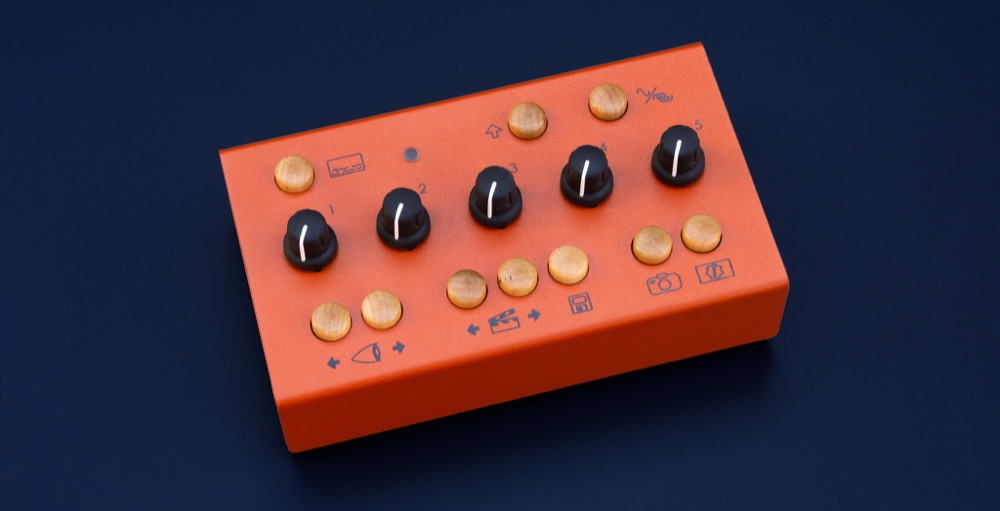
\includegraphics[width=0.75\linewidth,height=0.25\textheight,keepaspectratio]{images/critter-and-guitari-eyesy.jpg}
  \caption{Critter \& Guitari EYESY}
  \caption*{Retrieved from \cite{website-critter-and-guitari-current}}
  \label{fig:critter-and-guitari-eyesy}
\end{figure}

They can run on power supplies, and are also portable by the use of batteries.

\subsection{monome}

\begin{figure}[ht]
  \centering
  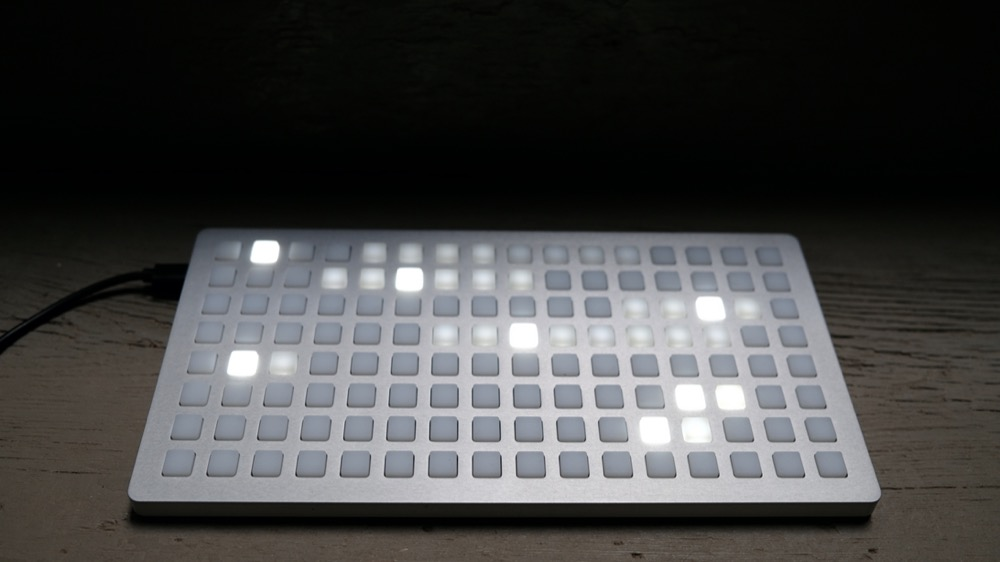
\includegraphics[width=0.75\linewidth,height=0.25\textheight,keepaspectratio]{images/monome-grid.jpg}
  \caption{monome grid}
  \caption*{Retrieved from \cite{website-monome-current}}
  \label{fig:monome-grid}
\end{figure}

Aleph: earlier sound computer.

Norns: sound computer, currently on its second iteration, with expanded hard drive. Also there is a \acrshort{DIY} version which is cheaper and runs on a Raspberry Pi.
Norns is a Linux machine, running SuperCollider for the sound engine, and Lua scripts. It has spawned a community that continually releases new scripts and software updates.

\begin{figure}[ht]
  \centering
  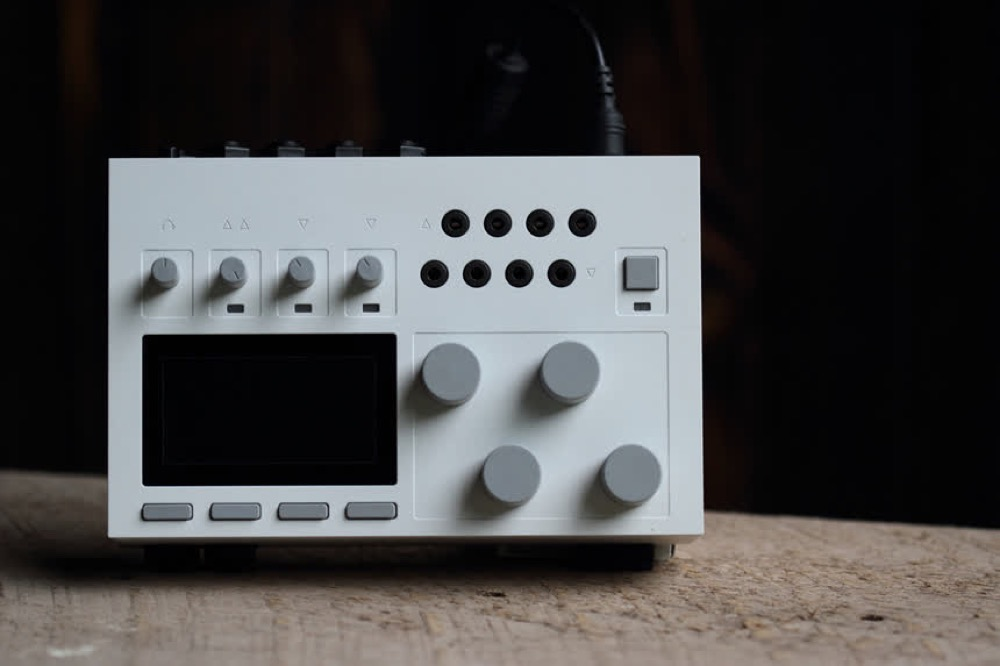
\includegraphics[width=0.75\linewidth,height=0.25\textheight,keepaspectratio]{images/monome-aleph.jpg}
  \caption{monome aleph}
  \caption*{Retrieved from \cite{website-monome-current}}
  \label{fig:monome-aleph}
\end{figure}

\begin{figure}[ht]
  \centering
  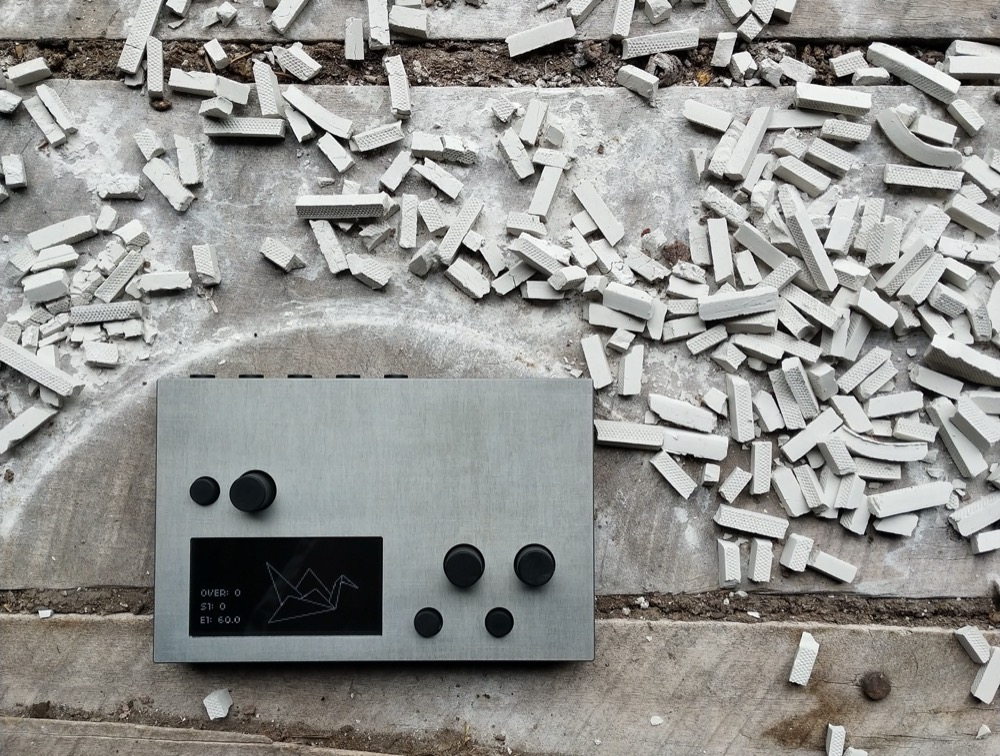
\includegraphics[width=0.75\linewidth,height=0.25\textheight,keepaspectratio]{images/monome-norns.jpg}
  \caption{monome norns}
  \caption*{Retrieved from \cite{website-monome-current}}
  \label{fig:monome-norns}
\end{figure}

\subsection{Shbobo}

In my first semester I was introduced by classmate Will Freudenheim to the Shbobo synthesizers by Peter Blasser. Peter Blasser has released several collections / companies of musical instruments, the most famous one being Ciat-Lonbarde.

\begin{figure}[ht]
  \centering
  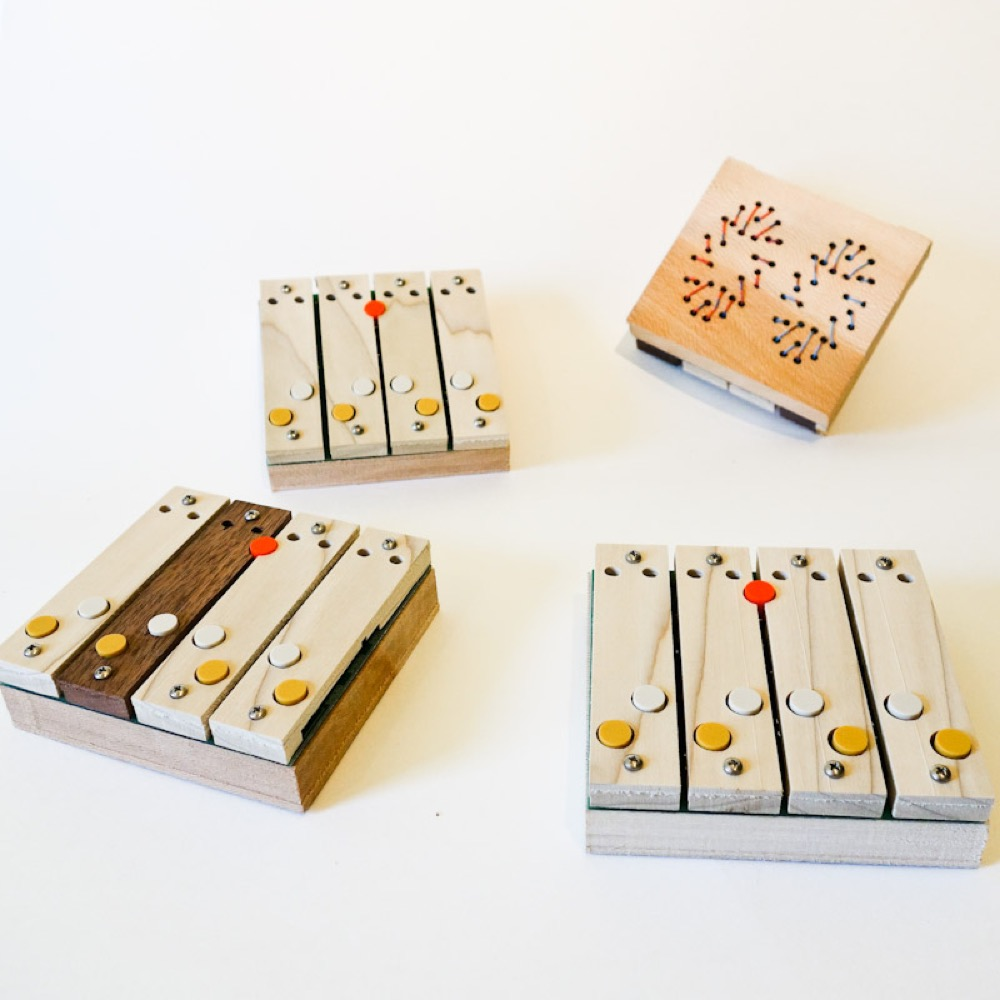
\includegraphics[width=0.75\linewidth,height=0.25\textheight,keepaspectratio]{images/shbobo-shnth.jpg}
  \caption{Shbobo Shnth}
  \caption*{Retrieved from \cite{website-shbobo-current}}
  \label{fig:shbobo-shnth}
\end{figure}

\begin{figure}[ht]
  \centering
    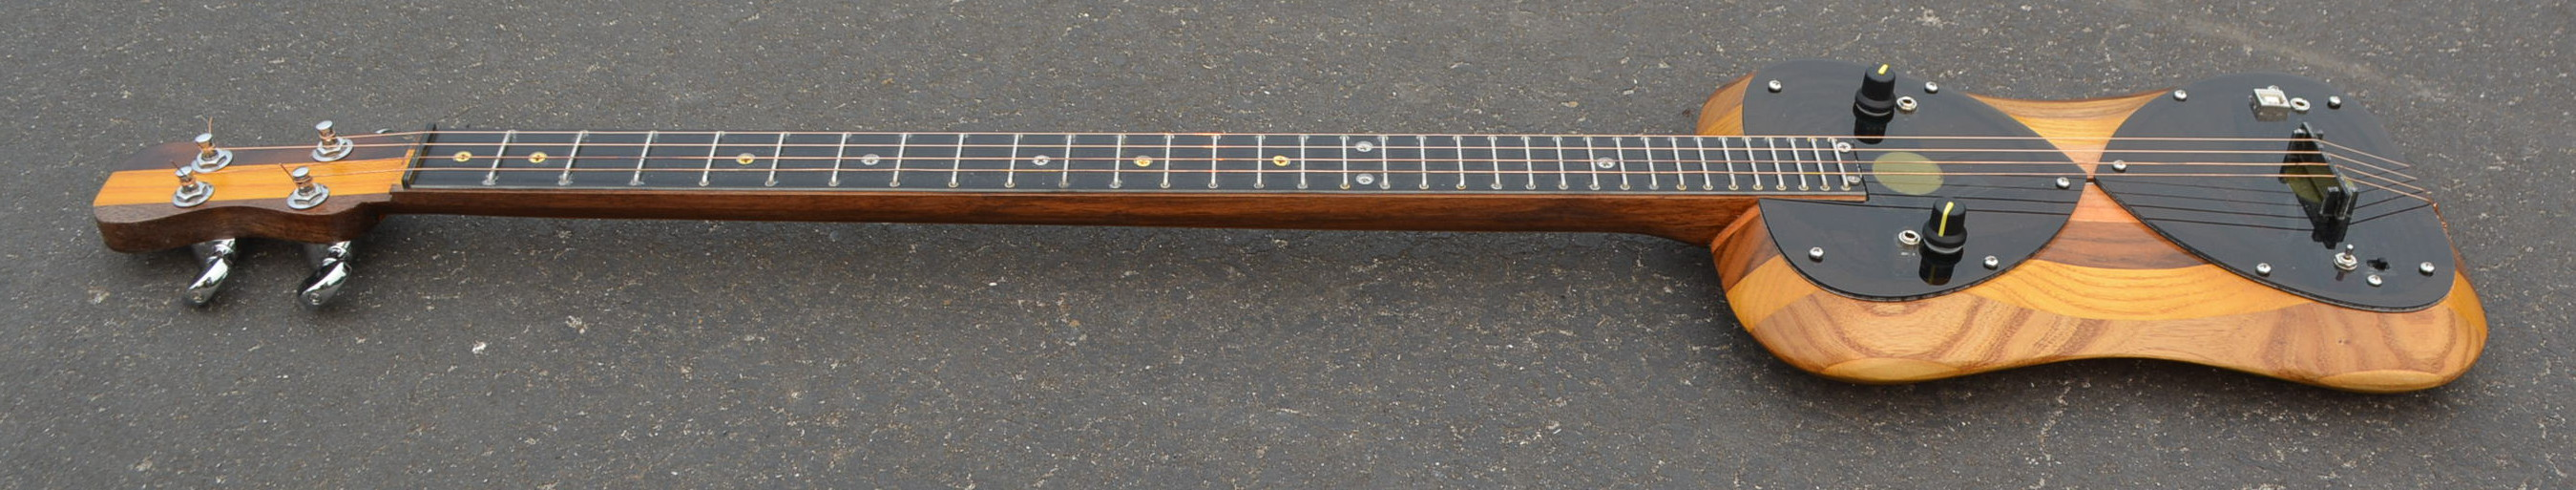
\includegraphics[width=0.75\linewidth,height=0.25\textheight,keepaspectratio]{images/shbobo-shtar.jpg}
  \caption{Shbobo Shtar}
  \caption*{Retrieved from \cite{website-shbobo-current}}
  \label{fig:shbobo-shtar}
\end{figure}

Both run on microcontrollers, and they use a new proposed language called Shlisp, based on Lisp, and also they can be programmed using the Fish IDE.

As of 2021, their firmware and editor became open source, and it is available at \url{https://github.com/pblasser/shbobo}.

COMMENT ON OPEN SOURCE: something being open source doesn't necessarily mean it is accessible to a wider audience. Is one of the goals of your work to create instruments that are accessible to a wider audience?

They promote computer-centric approaches to making sound, such as the use of integers and metaphors of finite state machines, and also allow for different ways of playing and sensing, such as the use of antennas for detecting hand distance, a microphone for detecting speech and whistling, and wooden bars with piezos for detecting pressure.

TODO: write how this inspired the new interactions i am inventing or appropriating for Tiny trainable instruments, such as a drum machine you can talk to, Alexa spinoff.

\section{Education}

This thesis is inspired by the work of the research group Lifelong Kindergarten at MIT Media Lab, led by professor Mitchel Resnick. In the book with the same title, he builds on Seymour Papert’s work, and proposes that educational projects should have “Low floor, wide walls, high ceilings”, and that learners thrive when they engage in the 4 Ps: “Peers, projects, passion, play”.

In terms of peers, I have been lucky to have been supported by the MIT UROP office and MIT Media Lab, and had the opportunity to work with MIT undergrad researchers Peter Tone and Maxwell Wang. Also, this project was taught in collaborative workshops where people could discuss their ideas with their peers.

In terms of projects, this thesis includes the release of a software library, so that people can make the software their own, and spin-off their own projects. It is also open source so that people can learn from my mistakes and also fork to adapt to their needs.

In terms of passion, this thesis is 

In terms of play, this thesis project is not about correct answers, or even excellent classification with \acrshort{ML}, it's all about finding innovative ways to interact with multimedia material, celebrate the small victories and the big glitches, and iterate over and over again.

\section{Creative ML}

COMMENT: what is the main argument of the whole piece and how does each independent part connect to that? you should start with a story from previous experiences that is particularly relevant as to why you were inspired to do this work. think "papert and the gears"

While being a graduate student and research resident at \acrshort{NYU} \acrshort{ITP} I saw how quick things changed in terms of \acrshort{ML}. I saw how the project deeplearn.js allowed for people to train and deploy \acrshort{ML} on their browsers, and how this library was acquired by Google and repurposed as TensorFlow.js, a JavaScript version of their \acrshort{ML} framework TensorFlow.

In turn, at \acrshort{NYU} \acrshort{ITP} a team of artists and programmers built the library and community of ml5.js, with the 5 being an homage to p5.js. Technically, ml5.js is a wrapper for TensorFlow.js, in the same spirit that p5.js is a wrapper for HTML5 elements such as the canvas.

\begin{figure}[ht]
  \centering
    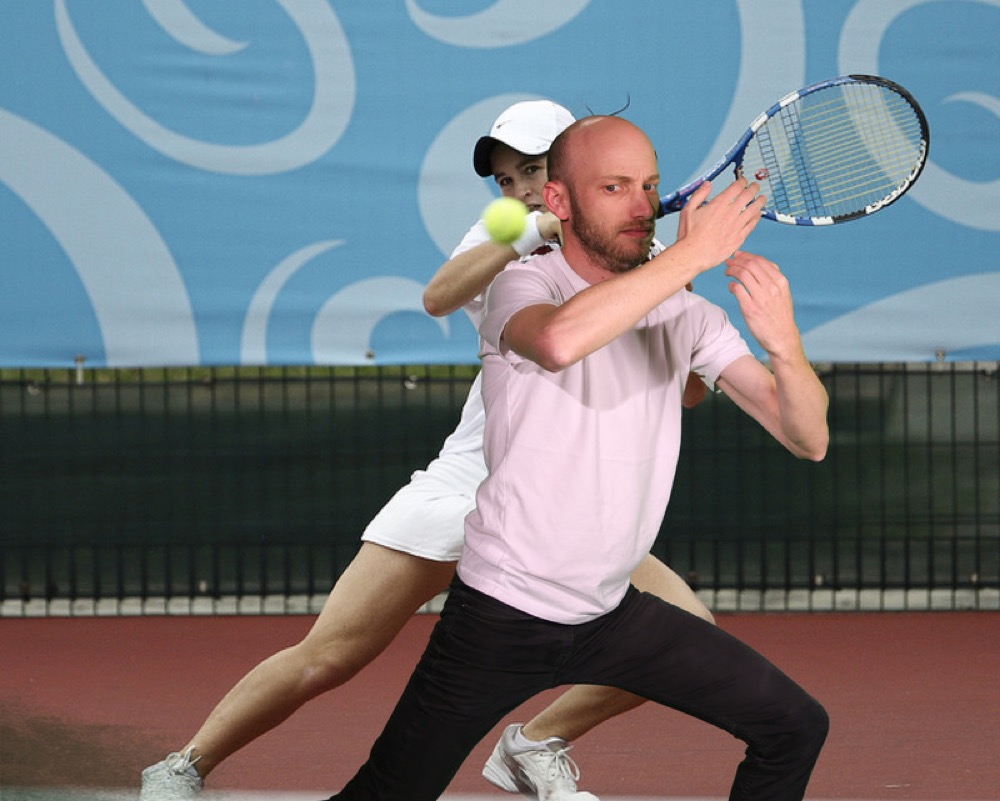
\includegraphics[width=0.75\linewidth,height=0.25\textheight,keepaspectratio]{images/sam-lavigne-training-poses.jpg}
  \caption{Sam Lavigne, Training Poses, 2018}
  \caption*{Retrieved from \cite{website-sam-lavigne-training-poses}}
  \label{fig:sam-lavigne-training-poses}
\end{figure}

The last spark that led me to this thesis was the release of 2 libraries for \acrshort{ML} on the Arduino platform: The currently beta version Arduino KNN, which allows for on-device training and resembles my earlier studies with Wekinator, in a more portable and private way, no data leaves the microcontroller, and the whole neural network can be wiped with one click of a button.

At a more complex level, I am also working with the TensorFlow Lite Micro, which I learned from Arduino blogs, and which currently is supported by the hardware Arduino Nano 33 \acrshort{BLE} Sense.

COMMENT TO THE ABOVE PARAGRAPH: you may not even need to include the specific details here, but just highlight in larger overviews the types of projects you've worked on or the educational fields that influence your work

In late 2020 and early 2021 I completed the just released series of 3 courses of the TinyML Professional Certificate by Harvard at the online platform edx.org

Newer books and references that this thesis was inspired by include the books “You Look Like a Thing and I Love You: How Artificial Intelligence Works and Why It's Making the World a Weirder Place” by Janelle Shane (2019), and the book “Making Pictures with Generative Adversarial Networks” by Casey Reas (2019).

Also Yining Shi created a new class at \acrshort{NYU} \acrshort{ITP} in 2020, at the intersection of \acrshort{ML} and physical computing.

\section{Digital rights}

\acrshort{ML} algorithms need data to be trained on. I think it’s a human right to not be surveilled, and I hope my thesis can put a positive spin on the gathering of data, by letting users perform auto surveillance, like the Ai Weiwei piece WeiweiCam, a 2021 project where the artist installed cameras for self surveillance as a protest against the Chinese government.

A huge inspiration for my thesis has been the Guardian Project by the Electronic Frontier Foundation, and the research and activism work by Sasha Sasha Costanza-Chock.

\section{Digital rights}

Electronic Frontier Foundation

Edward Snowden

Design Justice Network

\section{Opera of the Future projects}

During the development of this thesis, I have been fortunate to collaborate on different capacities with other thesis projects by classmates at Opera of the Future, which has directly inspired my work.

\subsection{Squishies, by Hannah Lienhard}

Squishies is Hannah Lienhard's Master's thesis, and consists of novel squishable interfaces for musical expression. We shared discussions about low-level sound design, code reusability, sound art education, and digital instruments. We were part of a Master's thesis working group, facilitated by Roya Moussapour with two other Media Lab classmates, where we workshopped drafts of our thesis. This practice and feedback has been critical in shaping the language and discourse of this thesis document.

\subsection{Fluid Music, by Charles Holbrow}

Fluid Music is Charles Holbrow's PhD thesis. It is a library for library design, documentation for contributors. The design of the interface, documentation, and scope of the thesis were a direct influence on the documentation and API coding style of this project.

TODO: mention the impact of the documentary Coded Bias, and how these researchers impacted my desire to make my thesis. Also mention how right before pandemic I had started a pottery class, with the intention of making clay-based instruments for thesis, as a metaphor of making code and hardware and software feel fluid and not static, I want to empower people to program, in particular \acrshort{ML} because of its dangerous implementations by oppressive governments and corporations, and in particular for arts, for making artists dream come true.
